\chapter{Executive Summary}
\label{ch:detectors-execsumm}

% Intro shared by all subsections

\section{An International Physics Program}

The global neutrino physics community is developing a multi-decade
physics program to measure unknown parameters of the Standard Model of
particle physics and search for new phenomena.  The program will be carried out as an international,
leading-edge, dual-site experiment for neutrino science and proton decay studies, which 
is known as the Deep Underground Neutrino Experiment (DUNE).
The detectors for this experiment will be designed, built, commissioned and operated by the international DUNE Collaboration. The facility required to support this experiment, the Long-Baseline Neutrino Facility (LBNF), is hosted by Fermilab and its design and construction is organized as a DOE/Fermilab project incorporating international partners. Together LBNF and DUNE will comprise the world's highest-intensity neutrino beam at Fermilab, in Batavia, IL, a high-precision near detector on the Fermilab site, a massive liquid argon time-projection chamber (LArTPC) far detector installed deep underground at the Sanford Underground Research Facility (SURF) \SI{1300}{\km} away in Lead, SD, and all of the conventional and technical facilities necessary to support the beamline and detector systems. 


The strategy for executing the experimental program presented in this Conceptual 
Design Report (CDR) has been developed to meet the requirements 
set out in the P5 report~\cite{p5report} and takes into account the recommendations of the European Strategy for Particle Physics~\cite{ESPP-2012}. It adopts a model where U.S. and international funding agencies 
share costs on the DUNE detectors, and CERN and other participants provide in-kind contributions 
to the supporting infrastructure of LBNF. LBNF and DUNE will be tightly coordinated as DUNE collaborators 
design the detectors and infrastructure that will carry out the scientific program.
  
The scope of LBNF is
\begin{itemize}
\item an intense neutrino beam aimed at the far site
\item conventional facilities at both the near and far sites
\item cryogenics infrastructure to support the DUNE
  liquid argon time-projection chamber (LArTPC) detectors at SURF
\end{itemize}

The DUNE detectors include
\begin{itemize}
\item a high-performance neutrino detector and beamline monitoring system
located a few hundred meters downstream of the neutrino source
\item a massive LArTPC neutrino detector located deep underground at the far site
\end{itemize}

With the facilities provided by LBNF and the detectors provided by
DUNE, the DUNE Collaboration proposes to mount a focused attack on the
puzzle of neutrinos with broad sensitivity to neutrino oscillation
parameters in a single experiment.  The focus of the scientific
program is the determination of the neutrino mass hierarchy and the
explicit demonstration of leptonic CP violation, if it exists, by
precisely measuring differences between the oscillations of muon-type
neutrinos and antineutrinos into electron-type neutrinos
and antineutrinos, respectively. Siting the far detector deep underground will
provide exciting additional research opportunities in nucleon decay,
studies utilizing atmospheric neutrinos, and neutrino astrophysics,
including measurements of neutrinos from a core-collapse supernova
should such an event occur in our galaxy during the experiment's
lifetime.

%%%%%%%%%%%%%%%%%%%%%%%%%%%%%%%%%%%%%%%%%%%%%%%%%%%%%%%%%%%%%%%
\section{The LBNF/DUNE Conceptual Design Report Volumes}

%%%%%%%%%%%%%%%%%%%%%%%%%%%%%%%%%%%
\subsection{A Roadmap of the CDR}

The LBNF/DUNE CDR describes the proposed physics program and 
technical designs at the conceptual design stage.  At this stage, the design is
still undergoing development and the CDR therefore presents a \textit{reference design} 
for each element as well as \textit{alternative designs} that are under consideration.

The CDR is composed of four volumes and is supplemented by several annexes that 
provide details on the physics program and technical designs. The volumes are as follows

\begin{itemize}
\item \volintro{} provides an executive summary of and strategy for the experimental 
program and of the CDR as a whole.
\item \volphys{} outlines the scientific objectives and describes the physics studies that 
the DUNE Collaboration will undertake to address them.
\item \vollbnf{} describes the LBNF Project, which includes design and construction of the 
beamline at Fermilab, the conventional facilities at both Fermilab and SURF, and the cryostat
 and cryogenics infrastructure required for the DUNE far detector.
\item \voldune{} describes the DUNE Project, which includes the design, construction and 
commissioning of the near and far detectors. 
\end{itemize}

More detailed information for each of these volumes is provided in a set of annexes listed on the \href{https://web.fnal.gov/project/LBNF/ReviewsAndAssessments/LBNF-DUNE%20CD-1-Refresh%20Directors%20Review/SitePages/Home.aspx}{review website}. 

%%%%%%%%%%%%%%%%%%%%%%%%%%%%%%%%%%%
%\subsection{About this Volume}  <----- follows in overview chapter file of indiv volume



\section{Introduction to the DUNE Detectors}
\label{sec:intro-dune-det}
\fixme{Anne adding some possible text from the link Andre provided; go ahead and remove if you prefer to start from scratch!}

\subsection{The Far Detector}
\label{sec:intro-dune-far-det}

The DUNE collaboration aims to deploy four 10-kt (fiducial mass) far detector modules based on the Liquid Argon Time Projection Chamber (LArTPC) technology. The viability of the basic LArTPC technology has been proven by ICARUS experiment. Neutrino interactions in liquid argon produce ionization and scintillation signals. While the basic detection method is the same, DUNE contemplates two options for the readout of the ionization signals: single-phase readout, where the ionization is detected using wire planes in the liquid argon volume; and the dual-phase approach, where the ionization signals are amplified and detected in gaseous argon above the liquid surface. 
%
The DUNE reference design, which implements a single-phase readout, is currently being validated in the 35-t prototype LAr detector at Fermilab. This design allows the charge to be collected directly, enabling precision calibration.
\fixme{Seems like we should say something about the reference design option first, then the alternate, so I changed the order.} The alternate design, employing a dual-phase approach, if demonstrated, would allow for a 3-mm readout pitch, a lower detection-energy threshold, and better pattern reconstruction of the events. A 20-t dual-phase readout prototype is being constructed at CERN and will operate in 2016. 

An active development program for both technologies is being pursued in the context of the Fermilab SBN program and the CERN neutrino platform. The development of the dual-phase technology is currently fully funded from outside the DOE project, although interest from DOE groups has been expressed in the context of the CERN Neutrino Platform. A flexible approach to the DUNE far detector design offers the potential to attract additional interest and resources into the Collaboration. The vision for the far detector is consolidated in line with \fixme{can we just say ``follows''?} the requirements set by the CD milestones and is guided by the following principles:

\fixme{I did some reorganization here, see what you think..}
\begin{itemize}
\item For the first 10-kt module, the Collaboration will adopt the lowest-risk design that satisfies the requirement and allows for installation at SURF to commence in 2021/2022. According to current plans, the first 10-kt module will implement the APA/CPA reference design, discussed in Section~\ref{sec:detectors-fd-ref-tpc}, subject to risks identified in the register.

\item Installation of the second 10-kt module should commence before 2023. The DUNE collaboration will instrument the second cryostat as soon as possible.

\item There is recognition that the LArTPC technology will continue to evolve with (1) the large-scale prototypes at the CERN Neutrino Platform and the experience from the Fermilab SBN program, and (2) the experience gained during the construction and commissioning of the first 10-kt module. 

\item It is assumed that all four detector modules will be similar but not necessarily identical. There will be a clear and transparent decision process for the design of the second and subsequent modules, allowing for implementation of evolved LArTPC technology. The decision will be based on physics performance, technical and schedule risks, costs, and funding opportunities.

\item A comprehensive list of synergies between the reference and alternative design has been identified and summarized in Chapter~\ref{ch:detectors-synergy}. Common solutions for DAQ, electronics, HV feed-throughs, and so on, will pursued and implemented, independent of the details of the TPC design. 
\end{itemize}

\fixme{Anne is inserting a possible figure}

\begin{cdrfigure}[3D models of the designs for the DUNE far detector]{FarDet-overview-SP}{3D models of the single-phase reference design (left) and the dual-phase alternate design (right) for the DUNE far detector to be located at the 4850L. }
\centering
\begin{minipage}[b]{1.0\textwidth}
\begin{center}
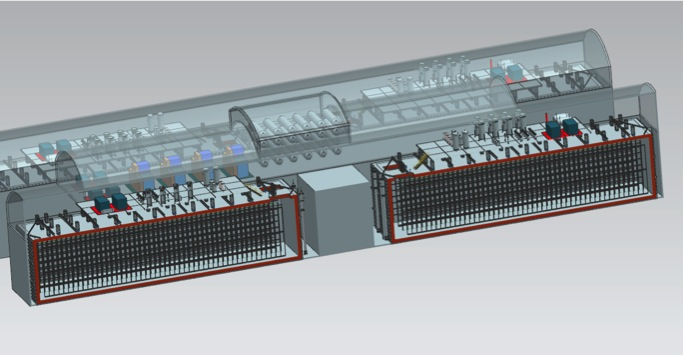
\includegraphics[width=.5\textwidth]{FarDet-3D-SP.jpg}
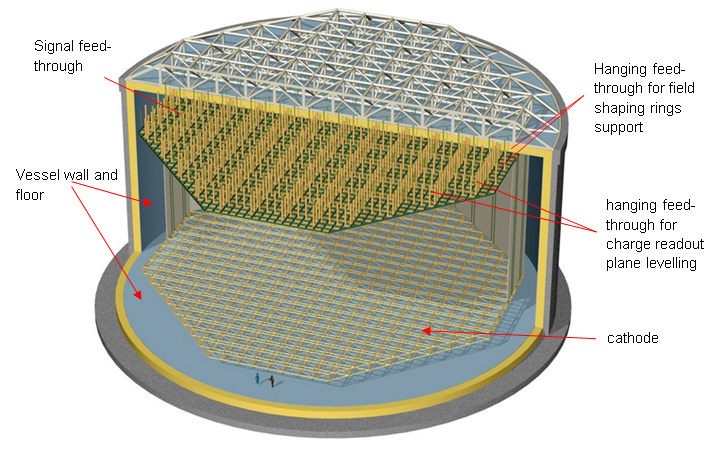
\includegraphics[width=0.46\textwidth]{LBNO50kton2}
\end{center}
\end{minipage}
\end{cdrfigure}

\subsection{The Near Detector}
\label{sec:intro-dune-near-det}

\fixme{I just copied some text; haven't looked at it...}

The primary scientific motivation for the DUNE near detector system is to constrain the beam spectrum for the long-baseline neutrino oscillation studies. It also provides high statistics for precision studies of neutrino-argon interactions. The near detector, which is exposed to an intense flux of neutrinos, also provides an opportunity for a wealth of fundamental neutrino interaction measurements, which are an important part of the secondary scientific goals of the DUNE collaboration. Within the former LBNE collaboration the neutrino near detector (NND) design was the NOMAD-inspired fine-grained tracker (FGT), which was built through a strong collaboration of U.S. and Indian institutes. Guiding principles for the near detector include

\begin{itemize}
\item Recognition of the central importance of the reference design for NND;

\item The primary design consideration of the DUNE neutrino near detector is the ability to adequately constrain the systematic errors in the DUNE LBL oscillation analysis;

\item The secondary design consideration for the DUNE NND is the self-contained non-oscillation neutrino physics program;

\item It is recognized that a detailed cost-benefit study of potential ND options has yet to take place and such a study is of high priority to the DUNE project. 
\end{itemize}

